\section{Results} \label{sec:resultados}

%Below are the results of solving a specific, simplified case, where the distance matrix corresponding to the road diagram in Figure \ref{fig:satelital} was obtained. Parameters for each well were generated randomly using a uniform distribution, assuming a particular initial regime and a target net battery production of $G_{dt}=335 m^3/\text{day}$ after reconfiguration. The distance and production parameters are presented in Tables \ref{tab:uno} and \ref{tab:dos}. The model was solved using the open-source solver SCIP \cite{scipto}, and the Pareto Frontier was generated by minimizing the maximum cumulative loss in the wells while bounding the distance to be traveled. Figure \ref{fig:dos} shows the results obtained. Table \ref{tab:sol} shows the bounded distance to minimize global loss with the new regimes adopted in each well based on the starting point represented by Table \ref{tab:dos}. Values highlighted in bold indicate those wells whose operating regimes were updated.

% \begin{table}[htb]
%     \centering
%     \scalebox{0.55}{
%     \begin{tabular}{|c|c|c|c|c|c|c|c|c|c|c|c|}
% \hline
% Wells&0&1&2&3&4&5&6&7&8&9&10\\
% \hline
%       0&  0	&1025&	927&	459&	955&	1481&	1307&	992&	964&	1332&	1457\\
% 1&1025	&0	&526&	842&	996&	1608&	446&	755&	1087&	1455&	1666\\
% 2&927	&526	&0	&468&	704&	1189&	532&	381&	713&	1081&	1292\\
% 3&459&	842&	468&	0&	496&	1108&	848&	533&	505&	873&	1084\\
% 4&955&	996&	704&	496&	0&	612&	1084&	769&	481&	377&	588\\
% 5&1481&	1608&	1189&	1108&	612&	0&	1466&	1254&	1093&	735&	270\\
% 6&1307&	446&	532&	848&	1084&	1466&	0&	761&	1093&	1461&	1672\\
% 7&992&	755&	381&	533&	769&	1254&	761&	0&	661&	1029&	1240\\
% 8&964&	1087&	713&	505&	581&	1093&	1093&	661&	0&	858&	1069\\
% 9&1332&	1455&	1081&	873&	377&	735&	1461&	1029&	858&	0&	711\\
% 10&1457&	1666&	1292&	1084&	588&	270&	1672&	1240&	1069&	711&	0\\
% \hline

%     \end{tabular}
%     }
%     \caption{Distances among all wells.``Well 0'' is the battery operations center.}
%     \label{tab:uno}
% \end{table}

% \begin{table}[htb]
%     \centering
% \scalebox{0.8} {
% \begin{tabular}{|c|c|c|c|}
% \hline
%    Well ($i$) &	Gross ($G_i$) $m^3/\text{day}$ &	Net ($N_i$) $m^3/\text{day}$ &	Regime ($r_i$) \% \\
% \hline
% 1&	60&	30&	82\\
% 2&	68&	35&	23\\
% 3&	75&	40&	18\\
% 4&	72&	40&	15\\
% 5&	63&	41&	27\\
% 6&	59&	58&	15\\
% 7&	62&	50&	24\\
% 8&	73&	42&	12\\
% 9&	68&	38&	12\\
% 10&	70&	51&	28\\
% \hline
%     \end{tabular}}
%     \caption{Initial parameters for the wells operation.}
%     \label{tab:dos}
% \end{table}

% \begin{table}[htb]
%     \centering
%  \scalebox{0.62}{  
%  \begin{tabular}{|p{1.2cm}|p{1cm}|c|c|c|c|c|c|c|c|c|c|}
%         \hline
%          \multirow{2}{*}{\parbox{1.2cm}{Dist. $m$}} & \multirow{2}{*}{\parbox{1cm}{Loss $m^3/\mbox{day}$}} &\multicolumn{10}{c|}{Well regime \%}\\
%          \cline{3-12}
%          &&1&2&3&4&5&6&7&8&9&10\\
%           \hline
        
%         2400 & 139.5 & 82 & 23 & \textbf{75.5} & \textbf{100} & 27 & 15 & 24 & \textbf{100} & 12 & 28\\
% 2617 & 128 & 82 & 23 & \textbf{94.3} & 15 & 27 & 15 & \textbf{100} & \textbf{100} & 12 & 28\\
% 3376 & 107.7 & \textbf{11.1} & \textbf{100} & \textbf{100} & 15 & 27 & \textbf{100} & \textbf{100} & 12 & 12 & 28\\
% 3857 & 103.8 & \textbf{0} & 23 & \textbf{93.1} & 15 & 27 & \textbf{100} & \textbf{100} & \textbf{100} & 12 & 28\\
% 4329 & 102.4 & \textbf{0} & 23 & \textbf{11.4} & \textbf{100} & 27 & \textbf{100} & \textbf{100} & \textbf{100} & 12 & 28\\
% 4851 & 97.5 & 82 & 23 & \textbf{0} & \textbf{62.8} & 27 & \textbf{100} & \textbf{100} & 12 & 12 & \textbf{100}\\
% 5309 & 90.4 & \textbf{0} & 23 & \textbf{0} & \textbf{62.3} & \textbf{100} & \textbf{100} & \textbf{100} & 12 & 12 & \textbf{100}\\
%         \hline
%     \end{tabular}
%     }
%     \caption{Working regimes for the wells minimizing the traveled distance.}
%     \label{tab:sol}
% \end{table}


\begin{figure}
    \centering
    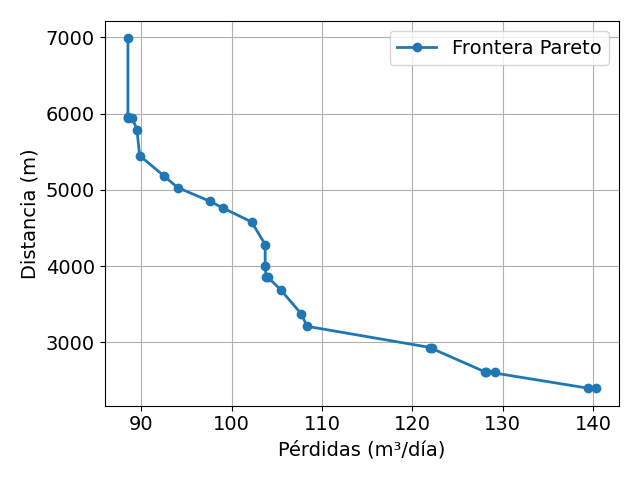
\includegraphics[scale=0.5]{imagenes/plot.png}
    \caption{Pareto's frontier for the example in Section~\ref{sec:resultados}.}
    \label{fig:dos}
\end{figure}